%% LaTeX2e Supplemential Instruction Template by Stephen Iota (https://stepheniota.com/)
%% last updated: May 2019
\documentclass[12pt]{article}
\usepackage{geometry}
%%%%%%%%%%%%%%%%
%%% Packages %%%
%%%%%%%%%%%%%%%%
\usepackage[utf8]{inputenc}
%\usepackage{tikz}
%\usepackage{lipsum}
\usepackage{amsmath,amssymb,amsfonts,physics}
\usepackage{graphicx}
\usepackage[shortlabels]{enumitem}
\usepackage[dvipsnames]{xcolor}
%\usepackage{footmisc}
%\usepackage{fancyhdr}
\usepackage[
	colorlinks=true,
	citecolor=NavyBlue!90!black,
	linkcolor=NavyBlue!75!black,
	urlcolor=green!50!black,
	hypertexnames=false]{hyperref}
 %%%%%%%%%%%%%%%%%%
 %% New Commands %%
 %%%%%%%%%%%%%%%%%%
\newcommand{\email}[1]{\texttt{\href{mailto:#1}{#1}}}
%%%%%%%%%%%%%%%%%%
%% Front Matter %%
%%%%%%%%%%%%%%%%%%
\graphicspath{{figures/}} % set directory for figures
\setcounter{section}{-1} % start with section 0
%%%%%%%%%%%%%
%%% Title %%%
%%%%%%%%%%%%%
\begin{document}
\begin{center}
\Large{Final Review}
\end{center}
\vspace{.5mm}
%%%%%%%%%%
%% INFO %%
%%%%%%%%%%
\begin{tabular}{rl}
\textsc{SI Leader}:			& 			Stephen Iota (\email{siota001@ucr.edu})
\\
\textsc{Course}:				&			Physics 40B (Spring 2019), Prof.~Barsukov
\\
\textsc{Date}:					&			\today
\end{tabular}
%%%%%%%%%%%%%%
%% PROBLEMS %%
%%%%%%%%%%%%%%

\section{History and snapshop graphs}

\begin{enumerate}[(a)]
\item Below is a snapshot graph at $t = 0$ sec for a wave moving to the right at a speed of 2.0 m/s. Draw a history graph for the position $x = 8.0$ m.
\begin{center}
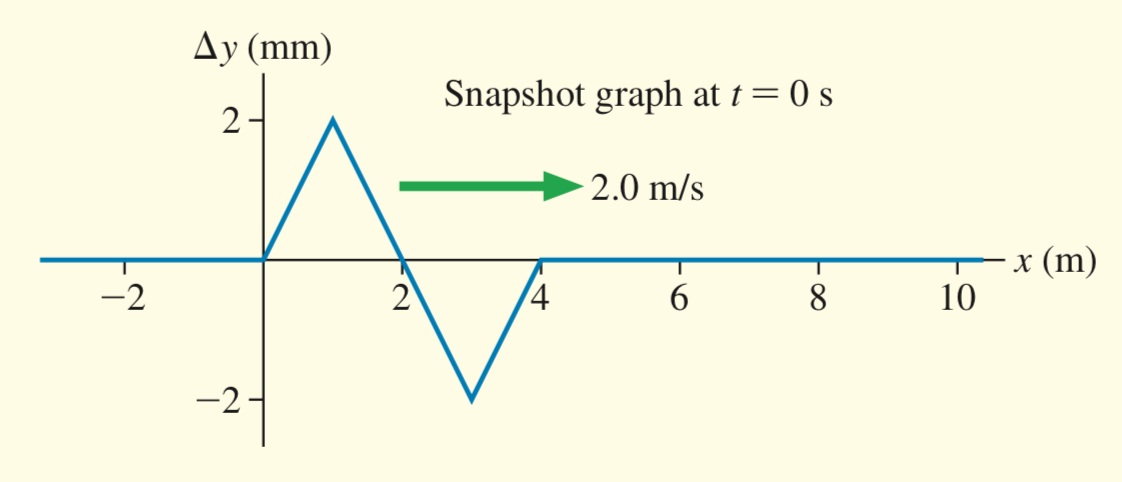
\includegraphics[width=.5\linewidth]{PSet4_FigA}
\end{center}

\item What is the frequency of the traveling wave below?
\begin{center}
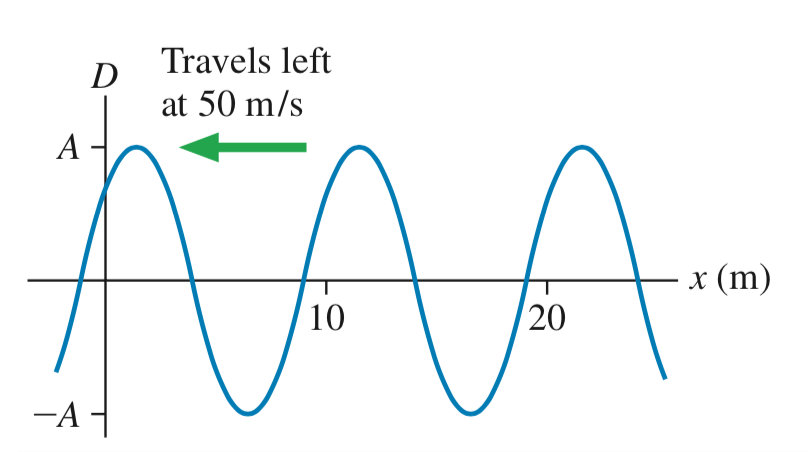
\includegraphics[width=.5\linewidth]{PSet4_FigB}
\end{center}
\end{enumerate}

\newpage
\section{Interference}

Two loudspakers emit sound waves along the $x$ axis. The sound has maximum intensity when the speakers are 20 cm apart. The sound intensity decreases as the distance between the speakers is increased, reaching zero at a separation of 60 cm.

\begin{enumerate}
\item What is the wavelength of the sound?
\item If the distance between the speakers continue to increase, at what separation will the sound intensity again be a maximum?s
\end{enumerate}


\newpage
\section{Doppler effect}

A physics professor demonstrates the Doppler effect by tying a 600 Hz sound generator to a 1.0 m long rope and whirling is around her head ina horizontal circle at 100 rpm. What are the highest and lowest frequencies heard by a student in the class room?

\newpage
\section{Laboratory}

The air temperature and pressure in a lab are 20 deg C and 1 atm. A 1.0 L containter is open to the air. The containter is then sealed and placed in a bath of boiling water. After reaching thermal equilibrium, the container is opened. How many moles of air escape?



\newpage
\section{Resonances in open-closed tubes}

\begin{figure}[h!]
\centering
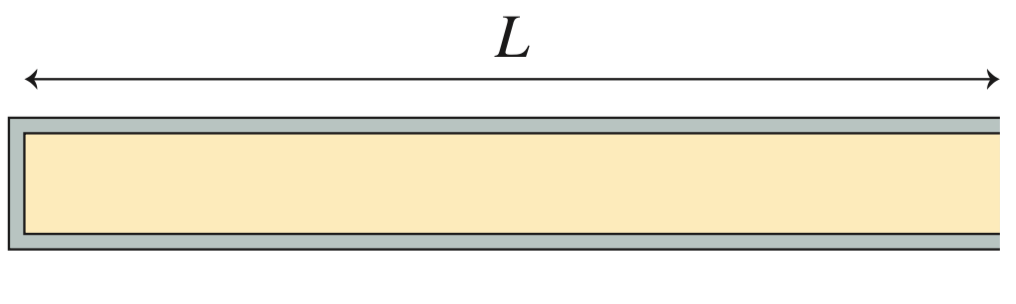
\includegraphics[width=.4\linewidth]{PSet5_Fig1}
\caption{Open-closed tube of length $L$.\label{tube}}
\end{figure}
\noindent
Let's think about what allowed modes of sounds waves are allowed in an open-closed tube such as in figure~\ref{tube}.
\begin{enumerate}[(a)]
\item Propose a general formula for the allowed wavelengths $\lambda_n$ and frequencies $f_n$ which generate standing waves in the open-closed tube.
\item How do the boundary conditions for this system differ from the closed-closed system discussed in lecture?
\end{enumerate}

\newpage
\section{Ideal gas processes}

A gas with initial state variables $P, V_1, T_1$ expands isothermally until $V_2 = 2V_1$. What are $T_2$ and $P_2$?

\newpage
\section{How much heat energy}

A monatomic gas fills the left end of the cylinder in the figure below. At 300K, the gas cylinder length is 10.0 cm and the spring is compressed by 2.0 cm. How much heat energy must be added to the gas to expand the cylinder length to 16.0 cm?

\begin{figure}[h!]
\centering
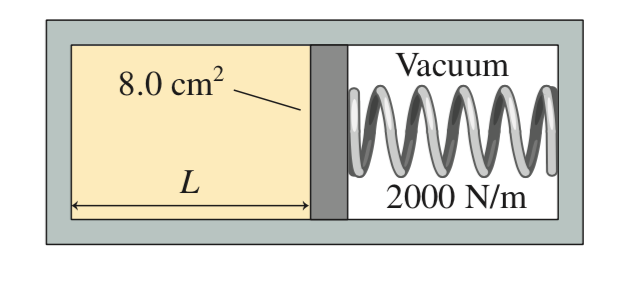
\includegraphics[width=0.5\linewidth]{Final_2}
\end{figure}


\newpage
\section{RMS speed}

The rms speed of the molecules in 1.0g of hydrogen gas is 1800 m$/$s.
\begin{enumerate}
\item What is the total translational kinetic energy of the gas of molecules?
\item What is the thermal energy of the gas?
\item 500 J of work are done to compress the gas while, in the same process, 1200 J of heat energy are transferred from the gas to the environment. Afterward, what is the rms speed of the molecules?
\end{enumerate}




\newpage
\section{Carnot heat engine and an ordinary fridge}

A Carnot heat engine and an ordinary refrigerator with coefficient of performance 2.00 operate between reservoirs at 350 K and 250 K. The work done by the Carnot heat engine drives the refrigerator. If the heat engine extracts 10.0 J of energy from the hot reservoir, how much energy does the refrigerator exhaust to the hot reservoir?



\newpage
\section{Heat engine driving fridge}

The figure below shows a Carnot heat engine driving a Carnot refrigerator.

\begin{enumerate}
\item Determine $Q_1, Q_2, Q_3$.
\item Is $Q_3$ greater than, less than, or equal to $Q_1$?
\item Does this apparatus violate the second law of thermodynamics?


\begin{figure}[h!]
\centering
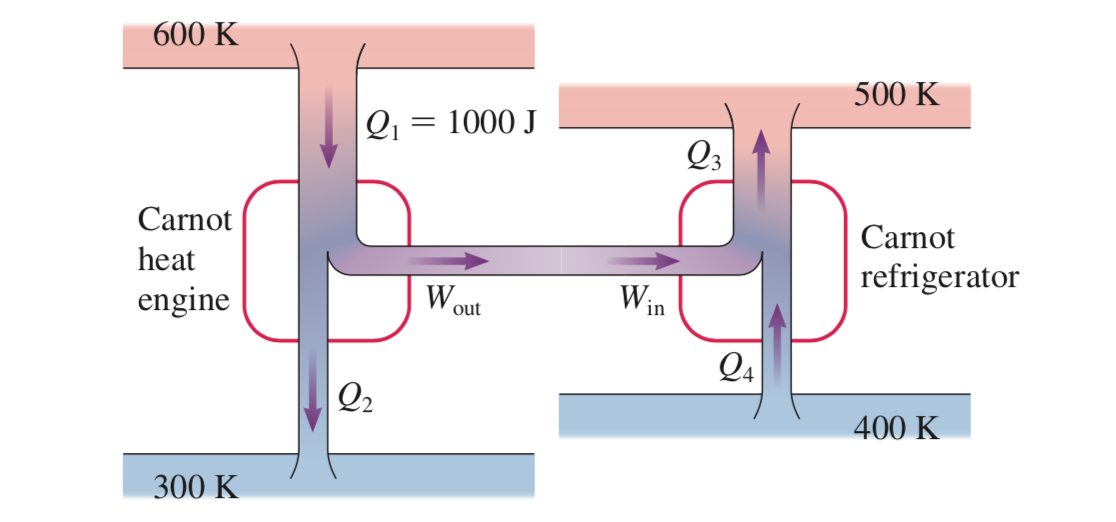
\includegraphics[width=0.5\linewidth]{Final_1}
\caption{Carnot heat engine driving Carnot fridge}
\end{figure}
\end{enumerate}








\end{document}
